\chapter{Present Simple and Present Continuous}

\begin{center}
\begin{tabular}{ccc}
\cefrlevel{A1-A2} & \textbf{Study Time:} 2-3 hours & \textbf{Difficulty:} ⭐⭐☆☆☆
\end{tabular}
\end{center}

\section{Lesson Objectives}
In this chapter, you will learn:
\begin{itemize}
    \item How to form and use the Present Simple tense
    \item How to form and use the Present Continuous tense
    \item The difference between routines (Present Simple) and actions happening now (Present Continuous)
    \item Stative verbs that don't use continuous forms
    \item Time expressions for each tense
\end{itemize}

\section{Reading Context}
\begin{readingbox}[title=Dialogue: A Typical Day vs. Right Now]
\textbf{Emma:} Hi Tom! What are you doing?\\
\textbf{Tom:} I\textbf{'m reading} a book about business. What about you?\\
\textbf{Emma:} I usually \textbf{work} in the office, but today I\textbf{'m working} from home.\\
\textbf{Tom:} That's nice. Do you \textbf{like} working from home?\\
\textbf{Emma:} Yes, I do. I \textbf{prefer} it because I \textbf{don't spend} time commuting.\\
\textbf{Tom:} I \textbf{understand}. The kids \textbf{are playing} outside right now, so it's quiet.\\
\textbf{Emma:} Perfect. By the way, what time do you usually \textbf{have} lunch?\\
\textbf{Tom:} I normally \textbf{eat} at 1 PM, but today I\textbf{'m having} lunch early.
\end{readingbox}

\begin{britishbox}[title=🇬🇧 British Daily Routines]
British people typically follow these routines:
\begin{itemize}
    \item \textbf{Breakfast:} 7-8 AM (cereal, toast, or a "full English breakfast")
    \item \textbf{Elevenses:} 11 AM (tea/coffee break - called "elevenses")
    \item \textbf{Lunch:} 12-1 PM (often called "dinner" in Northern England)
    \item \textbf{Tea time:} 4-5 PM (afternoon tea with biscuits or cake)
    \item \textbf{Dinner/Supper:} 6-8 PM (main evening meal)
\end{itemize}
\textbf{Fun fact:} British people drink an average of 3-4 cups of tea per day! ☕
\end{britishbox}

\section{Grammar Focus: Present Simple}

The Present Simple describes \textbf{routines, habits, facts, and general truths}.

\begin{grammarbox}[title=Present Simple Structure]
\textbf{Affirmative:}
\begin{itemize}
    \item I/You/We/They + \textbf{verb} (base form)
    \item He/She/It + \textbf{verb + s/es}
\end{itemize}

\textbf{Negative:}
\begin{itemize}
    \item I/You/We/They + \textbf{don't} + verb
    \item He/She/It + \textbf{doesn't} + verb
\end{itemize}

\textbf{Questions:}
\begin{itemize}
    \item \textbf{Do} + I/you/we/they + verb?
    \item \textbf{Does} + he/she/it + verb?
\end{itemize}

\textbf{Examples:}
\begin{itemize}
    \item I \textbf{work} in an office. \trans{Trabajo en una oficina}
    \item She \textbf{works} every day. \trans{Ella trabaja todos los días}
    \item They \textbf{don't like} coffee. \trans{No les gusta el café}
    \item \textbf{Does} he \textbf{speak} English? \trans{¿Habla inglés?}
\end{itemize}
\end{grammarbox}

\subsection{Spelling Rules for Third Person (he/she/it)}

\begin{table}[h]
\centering
\begin{tabular}{|l|l|l|}
\hline
\textbf{Rule} & \textbf{Example} & \textbf{Result} \\
\hline
Most verbs: add -s & work, play & works, plays \\
\hline
Ends in -s, -sh, -ch, -x, -o: add -es & wash, go, miss & washes, goes, misses \\
\hline
Ends in consonant + y: change to -ies & study, carry & studies, carries \\
\hline
Ends in vowel + y: add -s & play, enjoy & plays, enjoys \\
\hline
\end{tabular}
\caption{Third person singular spelling rules}
\end{table}

\section{Grammar Focus: Present Continuous}

The Present Continuous describes \textbf{actions happening now} or \textbf{temporary situations}.

\begin{grammarbox}[title=Present Continuous Structure]
\textbf{Structure:} Subject + \textbf{am/is/are} + \textbf{verb-ing}

\textbf{Affirmative:}
\begin{itemize}
    \item I \textbf{am working} (I'm working)
    \item He/She/It \textbf{is working} (He's working)
    \item We/You/They \textbf{are working} (They're working)
\end{itemize}

\textbf{Negative:}
\begin{itemize}
    \item I \textbf{am not} working (I'm not working)
    \item He \textbf{is not} working (He isn't working)
    \item They \textbf{are not} working (They aren't working)
\end{itemize}

\textbf{Questions:}
\begin{itemize}
    \item \textbf{Am} I working?
    \item \textbf{Is} he/she/it working?
    \item \textbf{Are} you/we/they working?
\end{itemize}

\textbf{Examples:}
\begin{itemize}
    \item I \textbf{am studying} right now. \trans{Estoy estudiando ahora}
    \item She \textbf{is reading} a book. \trans{Ella está leyendo un libro}
    \item They \textbf{aren't listening}. \trans{No están escuchando}
\end{itemize}
\end{grammarbox}

\subsection{Spelling Rules for -ING Forms}

\begin{table}[h]
\centering
\begin{tabular}{|l|l|l|}
\hline
\textbf{Rule} & \textbf{Example} & \textbf{Result} \\
\hline
Most verbs: add -ing & work, play & working, playing \\
\hline
Ends in -e: remove e, add -ing & make, write & making, writing \\
\hline
One syllable CVC: double consonant & sit, run, stop & sitting, running, stopping \\
\hline
Two syllables (stressed): double & begin, prefer & beginning, preferring \\
\hline
Ends in -ie: change to -ying & lie, die & lying, dying \\
\hline
\end{tabular}
\caption{Verb + -ing spelling rules}
\end{table}

\section{Key Differences: Simple vs. Continuous}

\begin{table}[h]
\centering
\begin{tabular}{|p{6cm}|p{6cm}|}
\hline
\textbf{Present Simple} & \textbf{Present Continuous} \\
\hline
Routines and habits & Actions happening now \\
\hline
I \textbf{go} to work by bus every day. & I \textbf{am going} to work by bus right now. \\
\hline
General truths and facts & Temporary situations \\
\hline
She \textbf{lives} in London. & She \textbf{is living} in a hotel this week. \\
\hline
Permanent situations & Actions in progress \\
\hline
He \textbf{works} in a bank. & He \textbf{is working} on a project. \\
\hline
\end{tabular}
\caption{Comparing Present Simple and Continuous}
\end{table}

\subsection{Visual Guide: When to Use Each Tense}

\begin{center}
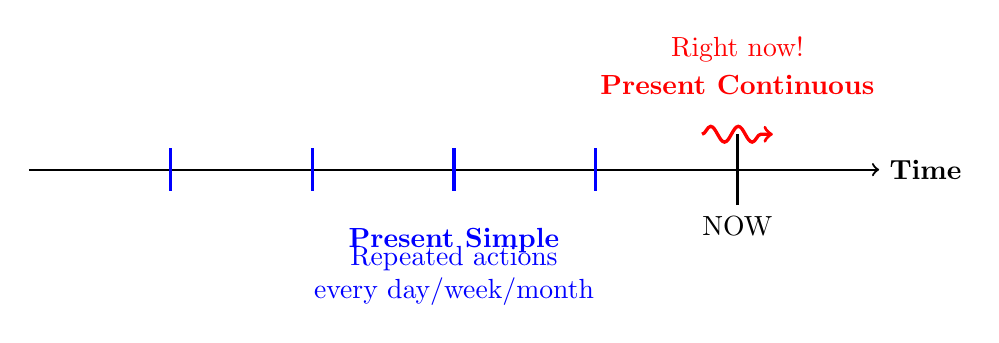
\begin{tikzpicture}[scale=0.9]
  % Timeline
  \draw[->, thick] (0,0) -- (12,0) node[right] {\textbf{Time}};
  
  % Present Simple - repeated actions
  \foreach \x in {2,4,6,8,10} {
    \draw[blue, very thick] (\x,-0.3) -- (\x,0.3);
  }
  \node[blue] at (6,-1) {\textbf{Present Simple}};
  \node[blue, align=center] at (6,-1.5) {Repeated actions\\every day/week/month};
  
  % Present Continuous - happening now
  \draw[red, very thick, ->, decorate, decoration={snake, amplitude=1mm}] (9.5,0.5) -- (10.5,0.5);
  \node[red] at (10,1.2) {\textbf{Present Continuous}};
  \node[red, align=center] at (10,1.7) {Right now!};
  
  % "Now" marker
  \draw[black, very thick] (10,-0.5) -- (10,0.5);
  \node[black] at (10,-0.8) {NOW};
\end{tikzpicture}
\end{center}

\begin{notebox}[title=💡 Quick Decision Guide]
Ask yourself: \textbf{Is it happening RIGHT NOW or is it a ROUTINE?}
\begin{itemize}
    \item Right now, at this moment → \textcolor{red}{\textbf{Present Continuous}}
    \item Every day, usually, always → \textcolor{blue}{\textbf{Present Simple}}
\end{itemize}
\end{notebox}

\section{Stative Verbs (No Continuous)}

Some verbs describe \textbf{states} (not actions) and are NOT normally used in continuous forms.

\begin{vocabbox}[title=Common Stative Verbs]
\begin{itemize}
    \item \textbf{Feelings:} like, love, hate, prefer, want, need
    \item \textbf{Thinking:} know, understand, believe, think (opinion), remember
    \item \textbf{Senses:} see, hear, smell, taste (involuntary)
    \item \textbf{Possession:} have (possess), own, belong
    \item \textbf{Being:} be, seem, appear
\end{itemize}

\textbf{Examples:}
\begin{itemize}
    \item I \textbf{like} pizza. \checkmark (NOT: I'm liking pizza. \textbf{X})
    \item She \textbf{knows} the answer. \checkmark (NOT: She's knowing. \textbf{X})
    \item We \textbf{have} a car. \checkmark (possession)
    \item We \textbf{are having} dinner. \checkmark (action - eating)
\end{itemize}
\end{vocabbox}

\section{Time Expressions}

\begin{table}[h]
\centering
\begin{tabular}{|l|l|}
\hline
\textbf{Present Simple} & \textbf{Present Continuous} \\
\hline
always, usually, often & now, right now, at the moment \\
sometimes, rarely, never & today, this week/month \\
every day/week/month & currently, at present \\
on Mondays, in the morning & Look!, Listen! \\
\hline
\end{tabular}
\caption{Common time expressions}
\end{table}

\section{Practice Exercises}

\subsection{Exercise 1: Present Simple - Fill in the Blanks}
Complete with the correct form of the verb in parentheses.

\begin{enumerate}
    \item She \underline{\hspace{3cm}} (work) in a hospital.
    \item They \underline{\hspace{3cm}} (not/like) spicy food.
    \item \underline{\hspace{3cm}} you \underline{\hspace{3cm}} (speak) French?
    \item He \underline{\hspace{3cm}} (go) to the gym every morning.
    \item We \underline{\hspace{3cm}} (not/watch) TV in the evening.
\end{enumerate}

\subsection{Exercise 2: Present Continuous - Fill in the Blanks}
Complete with the correct form of the verb in parentheses.

\begin{enumerate}
    \item I \underline{\hspace{3cm}} (read) a book right now.
    \item She \underline{\hspace{3cm}} (not/work) today.
    \item \underline{\hspace{3cm}} they \underline{\hspace{3cm}} (come) to the party?
    \item We \underline{\hspace{3cm}} (have) lunch at the moment.
    \item He \underline{\hspace{3cm}} (study) for his exam.
\end{enumerate}

\subsection{Exercise 3: Simple or Continuous?}
Choose the correct tense.

\begin{enumerate}
    \item I (work / am working) in London. I started this job 5 years ago.
    \item Look! It (rains / is raining).
    \item She (doesn't like / isn't liking) coffee. She prefers tea.
    \item What (do you do / are you doing)? I'm a teacher.
    \item What (do you do / are you doing) right now? I'm reading.
    \item I (think / am thinking) he's wrong. (opinion)
    \item I (think / am thinking) about my vacation. (process)
\end{enumerate}

\subsection{Exercise 4: Correct the Errors}
Find and correct the mistakes.

\begin{enumerate}
    \item She is liking chocolate very much.
    \item He go to school every day.
    \item Are you knowing the answer?
    \item I'm not understanding this lesson.
    \item They doesn't work on Sundays.
\end{enumerate}

\subsection{Exercise 5: Writing Task}
Write two paragraphs (60-80 words each):
\begin{enumerate}
    \item Describe your typical day (use Present Simple)
    \item Describe what you are doing today (use Present Continuous)
\end{enumerate}

\begin{tcolorbox}[colback=white,height=8cm]
% Paragraph 1: My typical day...

\vspace{3cm}

% Paragraph 2: What I'm doing today...
\end{tcolorbox}

\section{Common Mistakes to Avoid}

\begin{tcolorbox}[colback=red!5, colframe=red!60!black, title={Typical Errors}]
\begin{tabular}{|p{5cm}|p{5cm}|}
\hline
\textbf{❌ Incorrect} & \textbf{✓ Correct} \\
\hline
She \textcolor{red}{is liking} pizza. & She \textbf{likes} pizza. \\
\hline
He \textcolor{red}{go} to school. & He \textbf{goes} to school. \\
\hline
I \textcolor{red}{am knowing} him. & I \textbf{know} him. \\
\hline
They \textcolor{red}{doesn't} work. & They \textbf{don't} work. \\
\hline
She \textcolor{red}{work} every day. & She \textbf{works} every day. \\
\hline
What \textcolor{red}{you are doing}? & What \textbf{are you doing}? \\
\hline
I \textcolor{red}{am understand}. & I \textbf{understand}. \\
\hline
\end{tabular}
\end{tcolorbox}

\section{Quick Reference Card}

\begin{tcolorbox}[colback=blue!5, colframe=blue!60!black, title={Chapter Summary}]
\textbf{Key Points to Remember:}
\begin{itemize}
    \item \textbf{Present Simple:} routines, habits, facts → I work / She works
    \item \textbf{Present Continuous:} actions now, temporary → I'm working / She's working
    \item \textbf{Third person -s/-es:} work → works, go → goes, study → studies
    \item \textbf{Stative verbs:} like, know, understand, have (possession) → NO continuous
    \item \textbf{Time expressions:} always, usually (Simple) / now, right now (Continuous)
    \item \textbf{Questions:} Do you work? / Are you working?
\end{itemize}
\end{tcolorbox}

\section{Self-Assessment Checklist}

\begin{tcolorbox}[colback=green!5, colframe=green!60!black, title={✓ Can You Do This?}]
After studying this chapter, you should be able to:
\begin{itemize}
    \item[$\square$] Form positive sentences in Present Simple and Present Continuous
    \item[$\square$] Make negative sentences in both tenses
    \item[$\square$] Ask questions using Do/Does and Am/Is/Are
    \item[$\square$] Decide which tense to use (routine vs. now)
    \item[$\square$] Identify and use stative verbs correctly
    \item[$\square$] Apply the correct spelling rules for -s/-es and -ing
    \item[$\square$] Use appropriate time expressions with each tense
    \item[$\square$] Recognize and correct common mistakes
\end{itemize}

\textbf{💡 Study Tip:} If you can't check all boxes, review the relevant sections. Practice makes perfect!
\end{tcolorbox}

\section{Further Practice}

\begin{tipbox}[title=💡 How to Practice More]
\textbf{Speaking Practice:}
\begin{itemize}
    \item Record yourself describing your typical day (Present Simple)
    \item Narrate what you're doing right now (Present Continuous)
    \item Practice with a partner - ask and answer questions about routines
\end{itemize}

\textbf{Writing Practice:}
\begin{itemize}
    \item Keep a daily diary: "Today I am..." (Present Continuous)
    \item Write about your weekly routine (Present Simple)
    \item Describe what your family members usually do
\end{itemize}

\textbf{Listening Practice:}
\begin{itemize}
    \item Watch British TV shows or YouTube channels
    \item Listen to BBC podcasts about daily life
    \item Pay attention to how native speakers use these tenses
\end{itemize}

\textbf{Recommended Resources:}
\begin{itemize}
    \item BBC Learning English: "6 Minute Grammar"
    \item British Council LearnEnglish website
    \item Practice exercises at: www.perfect-english-grammar.com
\end{itemize}
\end{tipbox}

